\documentclass[a4paper,11pt]{exam}
	\usepackage{graphicx}
	\usepackage[utf8]{inputenc}
	\usepackage[T1]{fontenc}
	\usepackage{listings}
	\usepackage{color}
	\usepackage{amsmath}
	\usepackage{enumerate}
	\usepackage{caption}
	\usepackage{verbatim}
	\usepackage{subcaption}
	\usepackage{tikz}
	\usepackage{graphics}
	\usepackage{txfonts}
	\usepackage{listings}
	\definecolor{dkgreen}{rgb}{0,0.5,0}
	\definecolor{gray}{rgb}{0.5,0.5,0.5}
	\definecolor{mauve}{rgb}{0.58,0,0.82}

	\lstset{frame=tb,
	  language=Python,
	  aboveskip=3mm,
	  belowskip=3mm,
	  showstringspaces=false,
	  columns=flexible,
	  basicstyle={\small\ttfamily},
	  numbers=none,
	  numberstyle=\tiny\color{gray},
	  keywordstyle=\color{blue},
	  commentstyle=\color{dkgreen},
	  stringstyle=\color{mauve},
	  breaklines=true,
	  breakatwhitespace=true
	  tabsize=3
	  }
	

\begin{document}
\begingroup 
	  \bf \Large Eletromagnetismo\\
	  \indent \normalsize André Del Bianco Giuffrida
	\endgroup
	\\ \quad
	\\
	\large{
	\emph{Lista 1 \\ Ex 1}
	\\
	\\
	O campo elétrico em certa região do espaço é $\vec{E}(\vec{r}) = kr^3 \hat{r}$ em coordenadas esféricas, sendo k uma constante. \\
	(a) Encontre a densidade de carga $\rho(r)$ fonte deste campo.
	\\
	(b) Determine o potencial elétrico $V(r)$}
	\\
	\\
	
	\normalsize
	\begin{figure}[h]
		\centering
		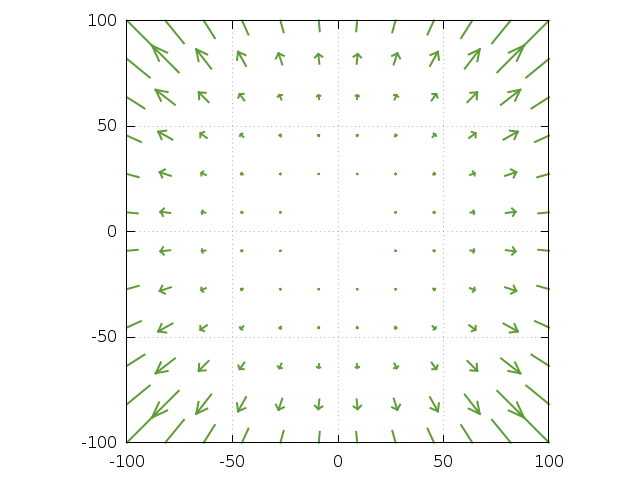
\includegraphics[scale=0.7]{Field2.png}
		\caption{ Campo $\vec{E}(\vec{r}) = kr^3 \hat{r}$}
	\end{figure}
	
	Partindo da definição de campo para uma distribuição de carga contínua
	
	\[\vec{E}(\vec{r}) = \frac{1}{4 \pi \epsilon_0} \int_{V} \frac{\hat R}{R^2}dq \quad \text{, onde } \quad R = \vec{r} - \vec{r'}\]
	
	Para uma densidade de carga espacial $\rho(\vec{r}) = \frac{dq}{dv}$
	
	\[ kr^3 \hat{r} = \frac{1}{4 \pi \epsilon_0} \int_{V} \frac{\hat R}{R^2} \rho(\vec{r'}) dv'\]
	
	\[ kr^3 \hat{r} = \frac{1}{4 \pi \epsilon_0} \int d\Omega \int_{0}^{\infty} \frac{\hat R}{R^2} \rho(\vec{r'}) dr'\]
	
	\[ kr^3 \hat{r} = \frac{1}{\epsilon_0} \int_{0}^{\infty} \frac{\hat R}{R^2} \rho(\vec{r'}) dr'\]
	
	Para resolver essa integral podemos usar o Divergente do campo.
	
	\[\nabla \cdot A = \frac{1}{r^2} \frac{\partial}{\partial r} (r^2 A_r) + \frac{1}{r sin(\theta)} \frac{\partial}{\partial \theta} (\sin(\theta)A_\theta) + \frac{1}{r\sin(\theta)} \frac{\partial A_\phi}{\partial \phi}\]
	
	\[ \frac{1}{r^2} \frac{\partial}{\partial r} (kr^5) = \nabla \cdot \frac{1}{\epsilon_0} \int_{0}^{\infty} \frac{\hat R}{R^2} \rho(\vec{r'}) dr'\]
	Aqui $\nabla$ atua na variavel $r$, podemos escrever:
	\[ 5kr^2 = \frac{1}{\epsilon_0} \int_{0}^{\infty} \nabla \cdot \Bigg[ \frac{\hat R}{R^2} \Bigg] \rho(\vec{r'})  dr'\]
	Usando a função delta de dirac ( $\delta$ )
	\[\nabla \cdot \Bigg[ \frac{\hat R}{R^2} \Bigg] =  \delta(\vec{r} - \vec{r'}) \quad \text{,}  \quad  5kr^2 \epsilon_0 = \int_{0}^{\infty} \delta(\vec{r} - \vec{r'}) \rho(\vec{r'})  dr' \]
	
	\[\quad \rho(\vec{r}) = 5kr^2 \epsilon_0 \]
	
	
	\begin{figure}[h]
		\centering
		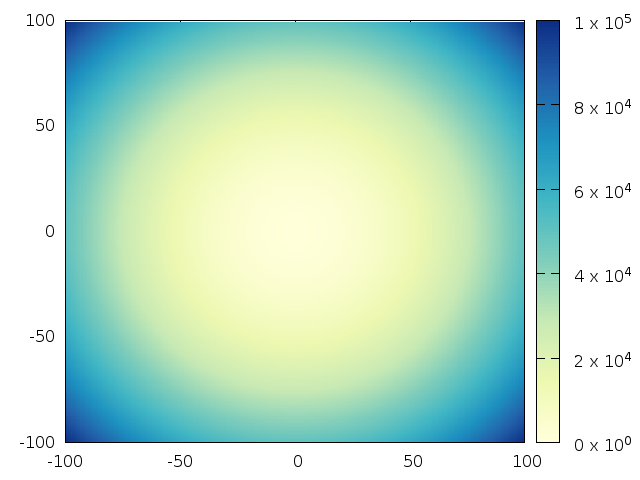
\includegraphics[scale=0.6]{Field1.png}
		\caption{Distribuição de Carga $\rho(\vec{r})$ em $\theta=\pi$}
	\end{figure}
	\pagebreak
	Agora para calcular $V(\vec{r})$ teremos que definir o referencial ($\vec{O_r}$) em um ponto arbitrário pois a densidade de carga se estende ao infinito! \\
	\indent Definindo $\vec{O_r} = (0,0,0)$ o que nos leva a:
	\[ V(\vec{r}) = - \int_{\vec{O_r}}^{\vec{r}}  \vec{E}(\vec{r}) \cdot d\vec{l} \quad = \quad - \int_{\vec{O_r}}^{\vec{r}}  kr^3 \hat{r} \cdot d\vec{l} \quad = \quad - \int_{0}^{r}  kr^3 dr\]
	\[ V(r) = - \frac{kr^4}{4}\Bigg|_{\vec{0}}^{\vec{r}} \quad \to \quad V(r) = - \frac{kr^4}{4} \]
	
	\begin{figure}[h]
		\centering
		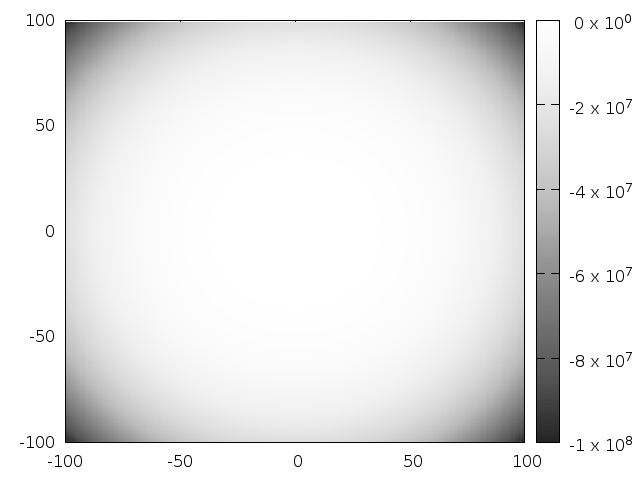
\includegraphics[scale=0.6]{Pot.png}
		\caption{Potencial $V(\vec{r})$}
	\end{figure}
	
	
	
\end{document}
